\section{\trJoyal{}特殊\trHorn{}提升定理}
\label{sec:joyal-special-horn-lifting}

本节我们从\trConservative{}函子（conservative functor）的概念出发，即一个检测给定的%
\trMorphism{}是否为\trEquivalence{}的\trFunctor{}。随后，我们将证明%
\trJoyal{}提升定理，该定理断言：\trConservative{}\trInnerFibration{}由相对于所谓特殊\trHorn{}%
（special horn）——即某条特定的边被送到\trEquivalence{}的那类\trHorn{}——的
提升性质刻画。由此，我们将推出∞-\trGroupoid{}是\trKanComplex{}，这是该理论
的中心结果之一。

\begin{definition}\label{def:conservative-functor}
∞-\trCategories{}之间的一个\trFunctor{} $F\colon \C \to \D$ 称为%
\emph{\trConservative{}}（conservative），如果它检测\trEquivalence{}，也就是说，如果只要
$f\colon x \to y$ 是 $\C$ 中的一个\trMorphism{}，使得 $F(f)\colon F(x) \to F(y)$
是 $\D$ 中的一个\trEquivalence{}，$f$ 本身便是一个\trEquivalence{}。
\end{definition}

\begin{observation}\label{obs:conservative-opposite}
\trFunctor{} $F\colon \C \to \D$ 是\trConservative{}，当且仅当其\trOppositeFunctor{}%
$F^{\mathrm{op}}\colon \C^{\mathrm{op}} \to \D^{\mathrm{op}}$ 是\trConservative{}。
\end{observation}

\begin{proposition}\label{prop:left-right-fibrations-conservative}
∞-\trCategories{}之间的\trLeftFibration{}与\trRightFibration{}是\trConservative{}。
\end{proposition}

\begin{proof}
通过过渡到相反范畴，只需处理\trLeftFibration{}的情形。设有\trMorphism{}%
$f\colon \Delta^1 \to \C$，它在 $\D$ 中成为一个\trEquivalence{}。考虑图表
\begin{center}
\begin{tikzpicture}
  \node (l) at (0,0) {$\Lambda^2_0$};
  \node (c) at (2.6,0) {$\C$};
  \node (d) at (0,-1.8) {$\Delta^2$};
  \node (r) at (2.6,-1.8) {$\D$};
  \draw[->] (l) -- (c);
  \draw[->] (l) -- (d);
  \draw[->] (c) -- node[right] {$p$} (r);
  \draw[->, dashed] (d) -- (r);
  \draw[->, dotted] (d) -- (c);
\end{tikzpicture}
\end{center}
其中映射 $\Lambda^2_0 \to \C$ 在边 $\Delta^{[0,1]}$ 上由 $f$ 给出，而在
$\Delta^{[0,2]}$ 上由恒等给出。由于 $\D$ 中的像是\trEquivalence{}，存在一条
虚箭头使图表交换。由于 $\C \to \D$ 是一个\trLeftFibration{}，点箭头也存在。
这证明 $f$ 在 $\C$ 中容有一个左逆，它在应用 $p$ 之后成为 $p(f)$ 的一个左逆，
从而在应用 $p$ 之后是一个\trEquivalence{}。对这个\trMorphism{}施以同样的
论证，可证明它自身容有一个左逆，这又表明最初构造的 $f$ 的那个左逆是一个%
\trEquivalence{}。因此，$f$ 也是一个\trEquivalence{}。
\end{proof}

\begin{definition}\label{def:isofibration}
∞-\trCategories{}之间的一个\trInnerFibration{} $\C \to \D$ 称为一个%
\emph{\trIsofibration{}}（isofibration），如果每个形如下述图表的\trLiftingProblem{}%
\begin{center}
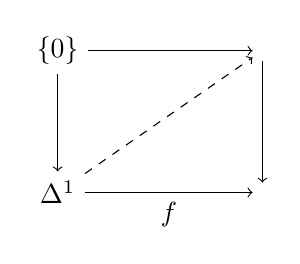
\begin{tikzpicture}
  \node (v) at (0,0) {$\{0\}$};
  \node (c) at (2.6,0) {$\C$};
  \node (d) at (0,-1.8) {$\Delta^1$};
  \node (r) at (2.6,-1.8) {$\D$};
  \draw[->] (v) -- (c);
  \draw[->] (v) -- (d);
  \draw[->] (c) -- (r);
  \draw[->] (d) -- node[below] {$f$} (r);
  \draw[->, dashed] (d) -- (c);
\end{tikzpicture}
\end{center}
其中 $f$ 代表 $\D$ 的一个\trEquivalence{}，都容有一个解，且该解代表 $\C$ 的
一个\trEquivalence{}。
\end{definition}

\begin{lemma}\label{lem:isofibration-homotopy-category}
∞-\trCategories{}之间的一个\trInnerFibration{} $\C \to \D$ 是\trIsofibration{}，当且仅当
诱导\trFunctor{} $\mathrm{N}(h\C) \to \mathrm{N}(h\D)$ 是\trIsofibration{}。
\end{lemma}

\begin{proof}
见\cref{ex:inner-fibration-isofibration}。
\end{proof}

\begin{corollary}\label{cor:isofibration-opposite}
∞-\trCategories{}之间的一个\trFunctor{} $\C \to \D$ 是\trIsofibration{}，当且仅当
$\C^{\mathrm{op}} \to \D^{\mathrm{op}}$ 是\trIsofibration{}。
\end{corollary}

\begin{proof}
见\cref{ex:isofibration-op}。
\end{proof}

\begin{proposition}\label{prop:left-right-fibrations-conservative-isofibrations}
∞-\trCategories{}之间的\trLeftFibration{}与\trRightFibration{}是\trConservative{}\trIsofibration{}。
\end{proposition}

\begin{proof}
由\cref{prop:left-right-fibrations-conservative}，\trLeftFibration{}与%
\trRightFibration{}是\trConservative{}。现在设 $p\colon \C \to \D$ 是一个%
\trLeftFibration{}，并考虑如\cref{def:isofibration} 中那般的一个%
\trLiftingProblem{}。由于 $\C \to \D$ 是一个\trLeftFibration{}，而
$\{0\} \to \Delta^1$ 是\trLeftAnodyne{}的，所需的提升存在。由保守性，任何这样
的提升都是一个\trEquivalence{}。对于\trRightFibration{}，使用%
\cref{cor:isofibration-opposite}。
\end{proof}

\begin{theorem}\label{thm:special-horn-lifting}
设 $\C \to \D$ 是∞-\trCategories{}之间的一个\trInnerFibration{}，并设
$\varphi\colon \Delta^1 \to \C$ 是 $\C$ 中的一个\trMorphism{}。那么对
$n \ge 2$，形如下述图表的\trLiftingProblem{}%
\begin{center}
\begin{tikzpicture}
  \node (d01) at (0,0) {$\Delta^{\{0,1\}}$};
  \node (horn) at (2.6,0) {$\Lambda^n_0$};
  \node (c) at (5.2,0) {$\C$};
  \node (dn) at (2.6,-1.8) {$\Delta^n$};
  \node (r) at (5.2,-1.8) {$\D$};
  \draw[->] (d01) -- (horn);
  \draw[->] (horn) -- (c);
  \draw[->] (horn) -- (dn);
  \draw[->] (c) -- (r);
  \draw[->] (dn) -- (r);
  \draw[->, dashed] (dn) -- (c);
\end{tikzpicture}
\end{center}
其中顶行的复合为 $\varphi$，只要 $\varphi$ 是 $\C$ 中的一个\trEquivalence{}，
便可求解。
\end{theorem}

\begin{proof}
为了在 $\varphi$ 是\trEquivalence{}这一假设下证明该提升性质，我们考虑图表
\begin{center}
\begin{tikzpicture}
  \node (d01) at (0,0) {$\Delta^{\{0,1\}}$};
  \node (horn) at (2.6,0) {$\Lambda^n_0$};
  \node (c) at (5.2,0) {$\C$};
  \node (dn) at (2.6,-1.8) {$\Delta^n$};
  \node (r) at (5.2,-1.8) {$\D$};
  \draw[->] (d01) -- (horn);
  \draw[->] (horn) -- (c);
  \draw[->] (horn) -- (dn);
  \draw[->] (c) -- (r);
  \draw[->] (dn) -- (r);
  \draw[->, dashed] (dn) -- (c);
\end{tikzpicture}
\end{center}
其中顶行复合是 $\C$ 中的一个\trEquivalence{}，设其为 $\varphi$，而我们希望
证明虚箭头的存在性。为此，我们观察到映射 $\Lambda^n_0 \to \Delta^n$ 同构于%
\trJoin{}--\trPushoutProduct{}%
\[
\{0\} \star \Delta^{-2+n} \amalg_{\{0\} \star \partial \Delta^{-2+n}}
\Delta^1 \star \partial \Delta^{n-2}
\longrightarrow
\Delta^1 \star \Delta^{-2+n},
\]
其中 $\Delta^{-2+n}$ 是 $\Delta^{\{2,\dotsc,n\}}$ 的简写形式。（这一结果见
\cref{ex:join-horn-computation}。）映射 $\Delta^{\{0,1\}} \to \Lambda^n_0$ 等同于典范复合
\[
\Delta^1 \longrightarrow \Delta^1 \star \partial \Delta^{-2+n}
\longrightarrow
\{0\} \star \Delta^{-2+n} \amalg_{\{0\} \star \partial \Delta^{-2+n}}
\Delta^1 \star \partial \Delta^{n-2}.
\]
经\trAdjunction{}，上图表等价于图表
\begin{center}
\begin{tikzpicture}
  \node (v) at (0,0) {$\{0\}$};
  \node (cs) at (6.1,0) {$\C_{/\Delta^{-2+n}}$};
  \node (d1) at (0,-1.6) {$\Delta^1$};
  \node (fp) at (4.6,-1.6)
    {$\C_{/\partial\Delta^{-2+n}} \times_{\D_{/\partial\Delta^{-2+n}}} \D_{/\Delta^{-2+n}}$};
  \node (c) at (6.1,-3.2) {$\C$};
  \draw[->] (v) -- (cs);
  \draw[->] (v) -- (d1);
  \draw[->, dashed] (d1) -- (cs);
  \draw[->] (d1) -- node[above] {$\phi'$} (fp);
  \draw[->] (d1) -- node[above, pos=0.45] {$\phi$} (c);
  \draw[->] (cs) -- (fp);
  \draw[->] (fp) -- (c);
\end{tikzpicture}
\end{center}
我们断言，图表
\begin{center}
\begin{tikzpicture}
  \node (a) at (0,0) {$\C_{/\Delta^{-2+n}}$};
  \node (b) at (4.4,0)
    {$\C_{/\partial\Delta^{-2+n}} \times_{\D_{/\partial\Delta^{-2+n}}} \D_{/\Delta^{-2+n}}$};
  \node (e) at (10.4,0) {$\C_{/\partial\Delta^{-2+n}}$};
  \node (f) at (13.2,0) {$\C$};
  \node (g) at (4.4,-1.6) {$\D_{/\Delta^{-2+n}}$};
  \node (h) at (10.4,-1.6) {$\D_{/\partial\Delta^{-2+n}}$};
  \draw[->] (a) -- (b);
  \draw[->] (b) -- (e);
  \draw[->] (e) -- (f);
  \draw[->] (b) -- (g);
  \draw[->] (e) -- (h);
  \draw[->] (g) -- (h);
\end{tikzpicture}
\end{center}
中三个顶行映射都是\trRightFibration{}，从而由%
\cref{prop:left-right-fibrations-conservative} 是\trConservative{}：第一个映射是%
\cref{thm:slice-fibration} 第 (1) 部分的对偶版本；最后一个映射显式陈述于
\cref{cor:slice-special-cases} 第 (1) 部分；而中间的映射是
$\D_{/\Delta^{-2+n}} \to \D_{/\partial\Delta^{-2+n}}$ 的一个\trPullback{}，
后者由与第一个映射相同的推理是\trRightFibration{}，故该\trPullback{}也是%
\trRightFibration{}。由 $\varphi$ 是\trEquivalence{}这一假设可知，$\varphi'$
也是\trEquivalence{}。于是虚箭头存在，因为由%
\cref{prop:left-right-fibrations-conservative-isofibrations}，
\trRightFibration{}是\trIsofibration{}。
\end{proof}

\begin{remark}\label{rem:special-horn-criterion}
对于 $\D = \Delta^0$，我们发现一个形如下述图表的\trLiftingProblem{}%
\begin{center}
\begin{tikzpicture}
  \node (d01) at (0,0) {$\Delta^{\{0,1\}}$};
  \node (horn) at (2.6,0) {$\Lambda^n_0$};
  \node (c) at (5.2,0) {$\C$};
  \node (dn) at (2.6,-1.8) {$\Delta^n$};
  \node (d0) at (5.2,-1.8) {$\Delta^0$};
  \draw[->] (d01) -- (horn);
  \draw[->] (horn) -- (c);
  \draw[->] (horn) -- (dn);
  \draw[->] (c) -- (d0);
  \draw[->] (dn) -- (d0);
  \draw[->, dashed] (dn) -- (c);
  \draw[->, bend left=40] (d01) to node[above] {$\phi$} (c);
\end{tikzpicture}
\end{center}
可求解，当且仅当 $\varphi$ 是一个\trEquivalence{}。「若」的情形刚刚已处理。
反之，假设任何这样的\trLiftingProblem{}都可求解。由 $n = 2$ 的情形，我们找到
$\varphi$ 的一个左逆 $\alpha$\footnote{译注：原书自此处起六处印作 $f$（「$\alpha$
是 $f$ 的左逆」、spine 限制 $(f,\alpha,f)$、$s_1(f)$、$s_0(f)$、「$f$ 的右逆」、
「$f$ 是等价」），而本注所述映射自陈述起即为 $\varphi$，未定义过任何 $f$，六处
径改。——译者注}，由一个 $2$-\trSimplex{} $\tau$ 所见证。于是我们
可以考虑 $\C$ 中的一个
$3$-\trHorn{}，其在\trSpine{}上的限制由 $(\varphi, \alpha, \varphi)$ 给出；
更精确地说，我们考虑映射 $\sigma\colon \Lambda^3_0 \to \C$，它具有下述诸面：
\begin{enumerate}[label=(\arabic*)]
  \item $\sigma|_{\Delta^{\{0,1,2\}}} = \tau$，
  \item $\sigma|_{\Delta^{\{0,1,3\}}} = s_1(\varphi)$，
  \item $\sigma|_{\Delta^{\{0,2,3\}}} = s_0(\varphi)$。
\end{enumerate}
那么，面 $\sigma|_{\Delta^{\{1,2,3\}}}$ 就是一个见证，表明 $\alpha$ 也是
$\varphi$ 的一个右逆，从而 $\varphi$ 是一个\trEquivalence{}。\footnote{译注：
$\Delta^{\{1,2,3\}}$ 并非 $\Lambda^3_0$ 的面；按原书本意，$\sigma$ 在此处指由
本假设（所述\trLiftingProblem{}皆可解，取 $n=3$）得到的扩张 $\Delta^3 \to \C$，其第
$0$ 个面即 $\sigma|_{\Delta^{\{1,2,3\}}}$。——译者注}
\end{remark}

\cref{thm:special-horn-lifting} 的一般情形读作如下。

\begin{corollary}\label{cor:conservative-special-horn}
∞-\trCategories{}之间的一个\trInnerFibration{} $p\colon \C \to \D$ 是\trConservative{}，
当且仅当对每个 $n \ge 2$ 与每个形如下述图表的\trLiftingProblem{}%
\begin{center}
\begin{tikzpicture}
  \node (d01) at (0,0) {$\Delta^{\{0,1\}}$};
  \node (horn) at (2.6,0) {$\Lambda^n_0$};
  \node (c) at (5.2,0) {$\C$};
  \node (dn) at (2.6,-1.8) {$\Delta^n$};
  \node (r) at (5.2,-1.8) {$\D$};
  \draw[->] (d01) -- (horn);
  \draw[->] (horn) -- (c);
  \draw[->] (horn) -- (dn);
  \draw[->] (c) -- node[right] {$p$} (r);
  \draw[->] (dn) -- (r);
  \draw[->, dashed] (dn) -- (c);
  \draw[->, bend left=40] (d01) to node[above] {$\phi$} (c);
\end{tikzpicture}
\end{center}
其中 $p(\varphi)$ 是 $\D$ 中的一个\trEquivalence{}，都存在一个解。
\end{corollary}

\begin{proof}
设 $p$ 是\trConservative{}。那么，$p(\varphi)$ 是\trEquivalence{}的假设便蕴含 $\varphi$
自身是\trEquivalence{}，从而任何这样的\trLiftingProblem{}都可由%
\cref{thm:special-horn-lifting} 求解。反之，设任何这样的\trLiftingProblem{}都
有解。为了证明 $p$ 是\trConservative{}，让我们考虑一个\trMorphism{}%
$\varphi\colon \Delta^1 \to \C$，使得 $p(\varphi)$ 是 $\D$ 中的一个%
\trEquivalence{}。考虑映射 $\Lambda^2_0 \to \C$，其在 $\Delta^{\{0,1\}}$ 上的
限制为 $\varphi$，而在 $\Delta^{\{0,2\}}$ 上的限制为恒等。由于 $\varphi$ 在
$\D$ 中变成一个\trEquivalence{}，\trLiftingProblem{}%
\begin{center}
\begin{tikzpicture}
  \node (d01) at (0,0) {$\Delta^{\{0,1\}}$};
  \node (horn) at (2.6,0) {$\Lambda^2_0$};
  \node (c) at (5.2,0) {$\C$};
  \node (dn) at (2.6,-1.8) {$\Delta^2$};
  \node (r) at (5.2,-1.8) {$\D$};
  \draw[->] (d01) -- (horn);
  \draw[->] (horn) -- (c);
  \draw[->] (horn) -- (dn);
  \draw[->] (c) -- node[right] {$p$} (r);
  \draw[->] (dn) -- (r);
  \draw[->, dashed] (dn) -- (c);
  \draw[->, bend left=40] (d01) to node[above] {$\phi$} (c);
\end{tikzpicture}
\end{center}
中的实线箭头便存在，\footnote{译注：原书本图中\trHorn{}印作 $\Lambda^n_0$（底为
$\Delta^n$），但据上文构造——限制在 $\Delta^{\{0,1\}}$ 上为 $\varphi$、在
$\Delta^{\{0,2\}}$ 上为恒等——此处应为 $n = 2$，兹改为 $\Lambda^2_0$（底为
$\Delta^2$）。——译者注}而它由假设可求解。这提供了 $\varphi$ 的一个左逆
$\psi$。如\cref{prop:left-right-fibrations-conservative} 的证明中那样，可知
$p(\psi)$ 是一个\trEquivalence{}。对 $\psi$ 施行同样的论证以代替 $\varphi$，
我们再次发现 $\psi$ 自身容有一个左逆，从而是一个\trEquivalence{}。因此，
$\varphi$ 也是一个\trEquivalence{}，从而 $p$ 是\trConservative{}。
\end{proof}

\begin{remark}\label{rem:opposite-special-horn}
包含映射 $\Delta^{\{0,1\}} \to \Lambda^n_0$ 的相反由映射
$\Delta^{\{n-1,n\}} \to \Lambda^n_n$ 给出。由于\trInnerFibration{}与\trConservative{}函子在
过渡到相反之下不变，我们发现：\cref{thm:special-horn-lifting} 与
\cref{cor:conservative-special-horn} 中把包含 $\Delta^{\{0,1\}} \to \Lambda^n_0$
替换为映射 $\Delta^{\{n-1,n\}} \to \Lambda^n_n$ 的类比陈述同样成立。
\end{remark}

注意，对我们而言，\cref{cor:conservative-special-horn} 中重要的方向是：只要
$p$ 是\trConservative{}，这样的\trLiftingProblem{}便可求解，正如下一个推论所示。

\begin{corollary}\label{cor:infinity-groupoids-kan}
∞-\trGroupoid{}是\trKanComplex{}。
\end{corollary}

\begin{proof}
由定义，∞-\trGroupoid{}恰好是那些典范映射 $\C \to \ast$ 为\trConservative{}%
∞-\trCategories{}。于是断言由\cref{cor:conservative-special-horn} 得出。
\end{proof}

现在我们处于可以定义∞-\trCategories{}的∞-\trCategory{}的位置：

\begin{definition}\label{def:cat-infinity}
∞-\trCategories{}的∞-\trCategory{} $\mathrm{Cat}_\infty$ 是如下%
\trSimplicialCategory{}的\trCoherentNerve{}：其\trObject{}为∞-\trCategories{}，
而其 hom-\trSimplicialSets{}由\trFunctor{}∞-\trCategory{} $\mathrm{Fun}(\C, \D)$
内部的极大子∞-\trGroupoid{}给出。（该定义依赖这样一个事实：极大子
∞-\trGroupoid{}的构造是从∞-\trCategories{}到\trKanComplex{}的一个幺半函子
（monoidal functor）：它是包含的\trRightAdjoint{}，从而保持乘积。）
\end{definition}

\begin{definition}\label{def:joyal-equivalence}
∞-\trCategories{}之间的一个\trFunctor{} $f\colon \C \to \D$ 是一个%
\emph{\trJoyalEquivalence{}}（Joyal equivalence，或称范畴等价（categorical
equivalence）），如果 $\mathrm{Cat}_\infty$ 中相应的 $1$-\trSimplex{}是
\cref{def:equivalence-infinity-category} 意义下的\trEquivalence{}。
\end{definition}

\begin{remark}\label{rem:joyal-equivalence-concretely}
具体地，这意味着存在一个 $2$-\trSimplex{}%
$\sigma\colon \Delta^2 \to \mathrm{Cat}_\infty$，使得
$\sigma|_{\Delta^{\{0,1\}}} = f$ 且 $\sigma|_{\Delta^{\{0,2\}}} = \mathrm{id}_{\C}$。由\cref{obs:simplicial-nerve-detail}，我们发现，对
$g = \sigma|_{\Delta^{\{1,2\}}}$，我们已在
$\mathrm{Fun}(\C, \D)^{\simeq}$ 中指定了一个从 $gf$ 到 $\mathrm{id}_{\C}$ 的
$1$-\trSimplex{}。换言之，$f$ 是一个\trEquivalence{}，当且仅当存在一个%
\trFunctor{} $g\colon \D \to \C$ 以及自然等价 $gf \simeq \mathrm{id}_{\C}$ 与
$fg \simeq \mathrm{id}_{\D}$，其意义见下一个定义。
\end{remark}

\begin{definition}\label{def:naturally-equivalent}
两个\trFunctor{} $f, f'\colon \C \to \D$ 称为\emph{（自然）等价的}%
（(naturally) equivalent），如果 $\mathrm{Cat}_\infty$ 中相应的\trMorphism{}是
\cref{def:equivalence-infinity-category} 意义下等价的。
\end{definition}

\begin{remark}\label{rem:equivalent-unwinding}
展开这些定义，我们发现：$f$ 与 $f'$ 等价，恰好当存在一个自然等价
$\tau\colon f \to f'$ 时成立，也就是说，$\tau$ 是∞-\trCategory{}%
$\mathrm{Fun}(\C, \D)$ 中 $f$ 与 $f'$ 之间的一个\trEquivalence{}。
\end{remark}

我们将继续给出\trJoyal{}扩张定理的更多应用。为此，回忆 $J$ 表示具有两个%
\trObject{} $0$ 与 $1$ 的可缩\trGroupoid{}。

\begin{corollary}\label{cor:equivalences-extend-over-j}
∞-\trCategory{} $\C$ 中的\trEquivalence{}恰好由那些在典范映射
$\Delta^1 \to J$ 上扩张的映射 $\Delta^1 \to \C$ 所表示。
\end{corollary}

\begin{proof}
「任何在 $J$ 上扩张的映射 $\Delta^1 \to \C$ 都是\trEquivalence{}」这一事实在
\cref{ex:extension-over-J-equivalence} 中讨论。反之，一个\trEquivalence{}由一个映射
$\Delta^1 \to \C^{\simeq} \subseteq \C$ 所表示。为了证明该映射在扩张
$\Delta^1 \to J$ 上扩张，由\cref{cor:infinity-groupoids-kan}，只需观察到
$\C^{\simeq}$ 是一个\trKanComplex{}，且映射 $\Delta^1 \to J$ 是\trAnodyne{}的。
（注意，其\trGeometricRealization{}是一个\trHomotopy{}等价，因为两者都可缩。）
关于该映射是\trAnodyne{}的这一事实的纯单纯证明，另见引理 2.4.5。
\end{proof}

\begin{corollary}\label{cor:pullback-conservative-inner-fibration}
∞-\trCategories{}之间的一个\trConservative{}\trInnerFibration{} $\C \to \D$ 沿任何%
\trFunctor{} $\D' \to \D$ 的\trPullback{}仍是一个\trConservative{}\trInnerFibration{}。
\end{corollary}

\begin{proof}
我们使用\cref{cor:conservative-special-horn} 所建立的\trConservative{}\trInnerFibration{}的
提升判据，并考虑图表
\begin{center}
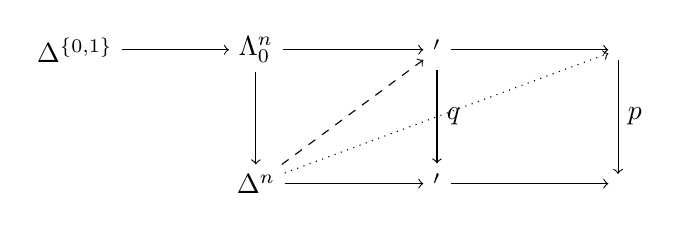
\begin{tikzpicture}
  \node (d01) at (0,0) {$\Delta^{\{0,1\}}$};
  \node (horn) at (2.3,0) {$\Lambda^n_0$};
  \node (cp) at (4.6,0) {$\C'$};
  \node (c) at (6.9,0) {$\C$};
  \node (dn) at (2.3,-1.7) {$\Delta^n$};
  \node (dp) at (4.6,-1.7) {$\D'$};
  \node (d) at (6.9,-1.7) {$\D$};
  \draw[->] (d01) -- (horn);
  \draw[->] (horn) -- (cp);
  \draw[->] (cp) -- (c);
  \draw[->] (horn) -- (dn);
  \draw[->] (cp) -- node[right] {$q$} (dp);
  \draw[->] (c) -- node[right] {$p$} (d);
  \draw[->] (dn) -- (dp);
  \draw[->] (dp) -- (d);
  \draw[->, dashed] (dn) -- (cp);
  \draw[->, dotted] (dn) -- (c);
\end{tikzpicture}
\end{center}
其中复合 $\Delta^1 \to \D'$ 代表一个\trEquivalence{}，而我们想要证明虚箭头
存在。由于 $p$ 是\trConservative{}，点箭头存在。于是，虚箭头也存在，因为右边的方形是
一个\trPullback{}。因此，$q$ 是\trConservative{}。
\end{proof}

\begin{proposition}\label{prop:isofibration-maximal-groupoid-kan}
∞-\trCategories{}之间的一个\trInnerFibration{} $p\colon \C \to \D$ 是\trIsofibration{}，
当且仅当诱导\trFunctor{} $\C^{\simeq} \to \D^{\simeq}$ 是一个\trKanFibration{}。
\end{proposition}

\begin{proof}
首先，设 $p$ 是\trIsofibration{}。作为第一步，我们证明诱导\trFunctor{}%
$p^{\simeq}\colon \C^{\simeq} \to \D^{\simeq}$ 也是一个\trIsofibration{}。为此，考虑
一个\trLiftingProblem{}%
\begin{center}
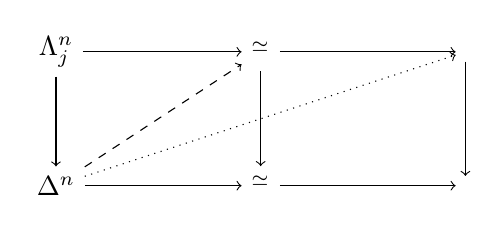
\begin{tikzpicture}
  \node (horn) at (0,0) {$\Lambda^n_j$};
  \node (cs) at (2.6,0) {$\C^{\simeq}$};
  \node (c) at (5.2,0) {$\C$};
  \node (dn) at (0,-1.7) {$\Delta^n$};
  \node (ds) at (2.6,-1.7) {$\D^{\simeq}$};
  \node (d) at (5.2,-1.7) {$\D$};
  \draw[->] (horn) -- (cs);
  \draw[->] (cs) -- (c);
  \draw[->] (horn) -- (dn);
  \draw[->] (cs) -- (ds);
  \draw[->] (c) -- (d);
  \draw[->] (dn) -- (ds);
  \draw[->] (ds) -- (d);
  \draw[->, dashed] (dn) -- (cs);
  \draw[->, dotted] (dn) -- (c);
\end{tikzpicture}
\end{center}
由于 $p$ 是一个\trInnerFibration{}，点箭头存在。我们断言，点箭头必定已经落入
$\C^{\simeq}$ 之中，从而产生出虚箭头。这由如下事实直接得出：它在\trSpine{}上
的限制落入 $\C^{\simeq}$，而这蕴含整个 $n$-\trSimplex{}都落在 $\C^{\simeq}$
之中。显然，$p^{\simeq}$ 满足\trIsofibration{}的进一步提升性质：该定义说，任何%
\trLiftingProblem{}%
\begin{center}
\begin{tikzpicture}
  \node (v) at (0,0) {$\{0\}$};
  \node (cs) at (2.6,0) {$\C^{\simeq}$};
  \node (c) at (5.2,0) {$\C$};
  \node (d1) at (0,-1.7) {$\Delta^1$};
  \node (ds) at (2.6,-1.7) {$\D^{\simeq}$};
  \node (d) at (5.2,-1.7) {$\D$};
  \draw[->] (v) -- (cs);
  \draw[->] (cs) -- (c);
  \draw[->] (v) -- (d1);
  \draw[->] (cs) -- (ds);
  \draw[->] (c) -- (d);
  \draw[->] (d1) -- (ds);
  \draw[->] (ds) -- (d);
  \draw[->, dashed] (d1) -- (cs);
\end{tikzpicture}
\end{center}
都有解。（我们只不过是明确指出：某些 $1$-\trSimplex{}被要求是\trEquivalence{}。）

接下来，我们观察到 $p^{\simeq}$ 显然是\trConservative{}，正如任何从∞-\trGroupoid{}出发的%
\trFunctor{}那样。因此，我们知道 $p^{\simeq}\colon \C^{\simeq} \to \D^{\simeq}$
既是一个\trConservative{}\trInnerFibration{}，又是一个\trIsofibration{}。为了看出它是一个%
\trKanFibration{}，我们先证明它是一个\trLeftFibration{}。左\trHorn{}%
$\Delta^0 \to \Delta^1$ 可以被扩张，因为 $p^{\simeq}$ 是一个\trIsofibration{}。对于
高维的左\trHorn{}，我们使用由\cref{cor:conservative-special-horn} 给出的\trConservative{}%
\trInnerFibration{}的判据，该判据告诉我们：只要\trHorn{}的某些边被映为%
\trEquivalence{}，提升就存在。但这个条件是重言式地满足的，因为 $\C^{\simeq}$
是一个∞-\trGroupoid{}。施行同样的论证（使用带右外\trHorn{}的\trJoyal{}提升
版本），我们还发现 $p^{\simeq}$ 是一个\trRightFibration{}，从而是一个%
\trKanFibration{}。

证明的逆方向是显然的：映射 $\{0\} \to \Delta^1$ 是一个\trHornInclusion{}，从而
对 $\C^{\simeq} \to \D^{\simeq}$ 容有一个提升，因为我们假设它是一个%
\trKanFibration{}。这表明 $p$ 是\trIsofibration{}。
\end{proof}

\begin{proposition}\label{prop:isofibration-rlp-j}
一个\trInnerFibration{} $\C \to \D$ 是\trIsofibration{}，当且仅当它对
$\Delta^0 \to J$ 具有\trRightLiftingProperty{}。特别地，\trIsofibration{}恰好是
\cref{def:joyal-fibration} 意义下∞-\trCategories{}之间的\trJoyalFibration{}。
\end{proposition}

\begin{proof}
显然，对 $\Delta^0 \to J$ 具有提升性质蕴含该映射是\trIsofibration{}。为了证明该论证的
逆方向，我们观察到每个图表
\begin{center}
\begin{tikzpicture}
  \node (d0) at (0,0) {$\Delta^0$};
  \node (c) at (2.6,0) {$\C$};
  \node (j) at (0,-1.7) {$J$};
  \node (d) at (2.6,-1.7) {$\D$};
  \draw[->] (d0) -- (c);
  \draw[->] (d0) -- (j);
  \draw[->] (c) -- (d);
  \draw[->] (j) -- (d);
\end{tikzpicture}
\end{center}
都分别穿过 $\C$ 与 $\D$ 的等价子范畴。因此，只需证明：一个映射
$f\colon \C \to \D$ 是\trIsofibration{}，当且仅当诱导映射
$\C^{\simeq} \to \D^{\simeq}$ 是一个\trKanFibration{}，而这已在%
\cref{prop:isofibration-maximal-groupoid-kan} 中完成。
\end{proof}

\begin{corollary}\label{cor:isofibration-stable-pullback}
\trIsofibration{}在\trPullback{}下稳定。
\end{corollary}
